Først vil det kort blive gennemgået, hvordan RSA virker, på matematisk niveau. Hvorefter der vil være et konkreteksempel.

\subsection{Matematisk protokol for RSA}\label{rsaprot}
Der følges igen i protokol, til fremstilling af den offentlige og den hemmelige nøgle.

\begin{enumerate}[label*=(\arabic*)] %[noitemsep]
    \item Udvælg 2 primtal \(p\) og \(q\), de skal gerne være omkring de 100 cifre hver og sæt så \(n = p \cdot q\)
    \item Udregn \(\phi(n)\), som er \((p - 1) (q - 1)\), da \(p\) og \(q\) er primtal.
    \item Vælg et tal \(e \in Z_{\phi(n)}^*\), altså sådan at \(0 < e < \phi(n)\) og \((e, \phi(n)) = 1\)
    \item Udregn det inverse element \(d\) til \(e \Mod{\phi(n)}\), sådan at \(e \cdot d \equiv 1 \Mod{\phi(n)}\). \label{stepfour}
\end{enumerate}

Når dette er gjort, er vi klar til at sende hemmelige beskeder.

\begin{itemize} %[noitemsep]
    \item Den offentlige nøgle er hhv. \(n\) og \(e\).
    \item Den hemmelige nøgle er \(d\).
\end{itemize}

Bemærk at \(p\) og \(q\) udelukkende er med til at generere \(n\) og \(\phi(n)\) og faktisk er \(\phi(n)\) også kun brug til at generere \(e\) og \(d\).
For at kunne bryde krypteringen, skal man kende \(d\) og \(d\) kan faktisk genereres ud fra den offentlige nøgle.\\
\emph{RSA bygger altså på antagelsen om, at det tager lang tid at primtalsfaktorisere \(n\)}
\par

Den besked \(m\) vi ønsker at sende, skal nu opfylde \(m < n\). Ellers må den opdeles i mindre bidder.

Beskeden \(m\), som skal sendes, krypteres ved at udregne \(c = m^e \Mod{n}\). \(c\) er nu den krypterde besked.

For at dekryptere \(c\), udregner man \(m = c^d \Mod{n}\)

\subsubsection{Bevis for RSA}
Det skal ses, hvorfor RSA virker, på baggrund af sætninger gennemgået i afsnit \ref{sec:numtheory}.
Krypteringen opskrives som en lang lighed.
\[c^d \Mod{n} = (m^e)^d \Mod{n} = m^{ed} \Mod{n} = m\]
Det sidste lighedstegn bevises.
\begin{proof}
        Der er to muligheder: \((m, n) = 1\) og \((m, n) \neq 1\).\\
        Kigger man på den første \((m, n) = 1\), ses det at ifølge sætning \ref{eulerssent} er \(m^{ed} \Mod{n} = m^{ed \Mod{\phi(n)}} \Mod{n}\).
        Og da \(e \cdot d = 1 \Mod{\phi(n)}\), som blev defineret ved step \ref{stepfour} i genereringen af tal.
        Ses det nu, at \(m^1 \Mod{n} = m\) hvorved det er bevist for \((m, n) = 1\).\\
        Beviset for \((m, n) \neq 1\) er noget længere og bygger på en del sætninger, som også tager tid at bevise, derfor bevises det blot hvordan der i forvejen er en meget lille sandsynlighed for at \((m, n) \neq 1\).\\
        Antag at \((m, n) \neq 1\), det må betyde at \(p \mid m \lor q \mid m\). Da \(m\) er genereret ud af de to primtal.
        De tal mellem 1 og \(n\), som gå op i \(m\), kan nu tælles:\\
        \(p\) går op i \(p, 2p, 3p, \hdots , (q - 1) \cdot p\).\\
        \(q\) går op i \(q, 2q, 3q, \hdots , (p - 1) \cdot q\).\\
        Der er derfor i alt \((p - 1) + (q - 1) + 1 = p + q - 1\), tal mellem 1 og \(n\) som går op i \(m\).
        Sammenlignes dette med antallet af tal i alt, mellem 1 og \(n\) -- antaget at \(p\) og \(q\) begge er på omkring de 100 cifre -- haves at.
        \[\frac{p + q - 1}{p \cdot q} \approx \frac{2 \cdot 10^{100}}{10^{200}} = 2 \cdot 10^{-100}\]
        Sandsynligheden for at \((m, n) \neq 1\), er altså minimal.\\
        Ønskes beviset for at ligheden er sand for \((m, n) \neq 1\), henvises der til Appendiks \ref{proofrsa}
\end{proof}


\subsection{RSA i aktion}
Vi skal nu tage et kig på hvordan RSA rent faktisk fungerer.
Tallene anvendt er naturligvis blot til eksempel -- i virkeligheden er de som sagt på omkring 100 cifre hver.\\

\begin{eks}
    Alice vil gerne logge på \url{https://www.netproever.dk/}, som Bob (staten) ejer, for at aflevere sin SOP, men på det netværk hun er forbundet til, sidder der nogle lumske typer, som gerne vil have fat i Alices kodeord, sådan at de kan logge ind som hende og aflevere noget bras.

    \begin{wrapfigure}{r}{0.5\textwidth}
        \vspace{-30pt}
        \begin{center}
            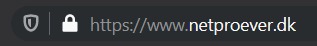
\includegraphics[width=0.48\textwidth]{img/secure.png}
        \end{center}
        \vspace{-20pt}
        \caption{Https og hængelås ud for URLen}
        \label{sikker}
        \vspace{-10pt}
    \end{wrapfigure}

    For at forhindre dette benytter Bobs website sig heldigvis af kryptering, hvilket også indikeres af browseren, hvor der står \texttt{https} oppe i søgebaren samtidig med at der er en hængelås før URLen -- se figur \ref{sikker}.
    \texttt{https} ``HyperText Transfer Protocol Secure'' er en protokol som lader browseren vide, hvordan den skal handle forespørgsler til websitet. \cite{https} Havde der blot stået \texttt{http}, ville forbindelsen ikke være krypteret. Det er altså vigtig at kigge på, inden man logger ind på en hjemmeside, for at undgå identitetstyveri.
    \par
    Det ses nu, hvordan Bob genererer en offentlig og en hemmelig nøgle ud fra protokollen fra afsnit \ref{rsaprot}.

    \begin{enumerate}[label*=(\arabic*)]%[noitemsep],leftmargin=1.5cm,series=example
        \item \(p = 41\) og \(q = 83\), \(n = 41 \cdot 83 = 3403\)
        \item \(\phi(n) = (41 - 1) (83 - 1) = 40 \cdot 82 = 3280\)
        \item \(e\) kan være mange værdier, men sættes i dette tilfælde til \(e = 43\)
        \item \(d\) beregnes til at være \(1907\), da \(1907 \cdot 43 \equiv 1 \Mod{3403}\)
    \end{enumerate}

    Kodeordet, som skal sendes omdannes til tal, ved at sætte \(A=01, B=02, C=03, \hdots , Z=26\), \(\_\) sættes til at være 00.
    Alices kodeord er tilfældigvis ``SOP\_OM\_RSA'', som omdannes til tal, vha. nævnte definition.
    Derudover deles beskeden op, sådan at hver bid, er mindre end \(n\), som er 3403.
    \begin{center}
        \begin{tabular}{l l l l l}
            S O  & P \_  & O M  & \_ R  & S A\\
            1915 & 1600  & 1513  & 0018   & 1901\\
        \end{tabular}
    \end{center}

    Nu tager Alice så fat i Bobs offentlig nøgle \((43, 3403)\), for at kryptere sit kodeord.
    For hver bid i hendes kodeord, skal hun udregne \(m^{43} \Mod{3403}\).
    Det ses, at allerede ved første bid, skal hun udregne \(1915^{43} \approx 1.35 \cdot 10^{141}\).
    Hvilket overgår de fleste lommeregneres kapacitet.
    Heldigvis kan \(m^{43}\) omskrives, vha potensregneregler. Hvorefter det er langt nemmere at udregne modulo.
    \begin{align*}
        m^{43} &= m \cdot m^{42}\\
        &= m \cdot (m^{21})^2\\
        &= m \cdot (m \cdot m^{20})^2\\
        &= m \cdot m^2 \cdot (m^{20})^2\\
        &= m \cdot m^2 \cdot ((m^{10})^2)^2\\
        &= m \cdot m^2 \cdot (((m^5)^2)^2)^2\\
        &= m \cdot m^2 \cdot (((m \cdot m^4)^2)^2)^2\\
        &= m \cdot m^2 \cdot ((m^2)^2)^2 \cdot (((m^4)^2)^2)^2\\
        &= m \cdot m^2 \cdot ((m^2)^2)^2 \cdot ((((m^2)^2)^2)^2)^2\\
    \end{align*}
    Beregningen udføres nu blot med henhold til sætning \ref{modmod}, sådan at der foretages en modulo operation, for hvert potens-led.
    Det ville fylde alt for meget at vise her, hvorfor det overlades til læseren. Alternativt er der et fint eksempel i. \cite[104]{krypto}
    \par
    Krypteringen udføres, for at få den krypterede besked.
    Dette kan også gøres i Python med kommandoen \texttt{pow()}\footnote{\url{https://docs.python.org/3/library/functions.html\#pow}}
    \begin{minted}[fontsize=\footnotesize, bgcolor=bg]{python}
>>>pow(base, exp[, mod])
    \end{minted}

    \begin{align*}
        1915^{43} \Mod{3403} &= 2454\\
        1600^{43} \Mod{3403} &= 944\\
        1513^{43} \Mod{3403} &= 469\\
        18^{43} \Mod{3403}   &= 174\\
        1901^{43} \Mod{3403} &= 2637\\
    \end{align*}

    Det ses altså, at de krypterede bidder, på ingen måde minder om de originale bidder.
    Krypteringen er på denne måde lykkedes og Alice kan trygt sende den krypterede besked over netværket.
    Når beskeden så lander ved Bob, som jo er den eneste, der kender \(d\), vil han kunne dekryptere den, validere at det er Alices' kodeord og derefter logge hende ind.

    Dekrypteringen foregår som sagt ved at udregne \(c^d \Mod{n}\).
    \begin{align*}
        2454^{1907} \Mod{3403} &= 1915\\
        944^{1907} \Mod{3403}  &= 1600\\
        469^{1907} \Mod{3403}  &= 1513\\
        174^{1907} \Mod{3403}  &= 0018\\
        2637^{1907} \Mod{3403} &= 1901
    \end{align*}

    Det er hermed vist, ved et eksempel, hvordan RSA virker.
\end{eks}



\subsection{UNI•Login}
Vi skal kigge lidt på sikkerheden ved en almindelig login-formular og se hvilke faktoere der spiller ind.
I de sidste mange år, har et UNI-login brugernavn, været de første 4 bogstaver i ens navn, efterfulgt af 4 tal (eller evt. bogstaver).
Mens koden har bestået af 3 små bogstaver, 2 tal efterfulgt af atter 3 bogstaver.
Men det skal langt om længe laves om. \cite{unilogin}
Set fra onlinesikkerhedens synspunkt, var det heller ikke et øjeblik for tidligt, da det som vist i afsnit \ref{kodeord}, er meget let at brute-force sig frem til så korte kodeord.
Den nye ordning, gør at der bl.a. skal være \emph{2FA}.\footnote{Engelsk for \emph{Two Factor Authentication}, betyder at man ikke blot skal logge ind med et fast kodeord, men også have noget seperat, som f.eks. nøglekortet til NemID, eller en engangskode tilsendt på SMS.}
Dette er naturligvis med til at øge sikkerheden voldsomt, da der er en variabel med inde over loginnet og ikke længere kun et fast brugernavn + kodeord.
Der er hovedsageligt 4 faktoere, som spiller ind på sikkerheden af en login-formular

\begin{enumerate}[noitemsep]
    \item En krypteret forbindelse, til formularen (RSA)
    \item Om loginnet er sat op til 2-faktor login
    \item Styrken af brugerens kodeord, herunder længde og kompleksitet
    \item Om kodeordet bliver hashet, herunder hvilken hashfunktion, samt brug af salt
\end{enumerate}


Udover faktor nummer 3, kan det, som bruger være svært at gøre noget ved nogle af disse foranstaltninger.
Derfor er det vigtigt at tjekke om siden man besøger er krypteret og så vidt muligt at forsøge at vælge et langt unikt kodeord eller bruge en \emph{password manager}.\footnote{En password manager kan selv generere og holde styr på dine kodeord. Kodeordene er så beskyttet af et master kodeord, som du selv skal huske, da det er ``nøglen'' til alle kodeordene. \href{https://www.lastpass.com/}{LastPass} og \href{https://www.dashlane.com/}{dashlane} er begge password managers.}

\subsection{Hvis vi ikke havde RSA}
Vores verden ville formentlig gå helt i stå, hvis vi en stod i den uheldige situation, at der blev fremvist en metode til at bryde RSA krypteringen.
Faktisk er der fremvist beviser for, at kvantecomputere, er langt bedre til at primtalsfaktorisere, end nudagens computere.\cite{quantum}
Heldigvis formår de samtidig at skabe en ny kryptering, som de ikke selv kan bryde.
Det er dog ikke noget, der vil blive taget yderligere op i denne tekst.

RSA er grundlag for al online-sikkerhed i dag, herunder autentificering, anonymisering og som sikkerhedsforanstaltning.
Hvis vi ikke havde RSA, ville ingen internettraffik længere være sikker, man ville ikke kunne stole på noget man læser online længere, da man ikke kan verificere udgiveren.
Samtidig ville det være dumt at give sig til kende, da alle på den måde, vil få fat i ens oplysninger på det åbne net.

Vi bør altså være glade for at RSA er opfundet, til at holde os sikre på nettet. Ikke kun i forbindelse med logins, men i den generelle færden på internettet.
